\documentclass[10pt, pdf, hyperref={unicode}]{beamer}
\usepackage[utf8]{inputenc}
\usepackage[russian]{babel}
\usepackage{graphicx}
\usepackage{wrapfig}
\usepackage{xcolor}
\usepackage{verbatim}
\usetheme{Berlin}
\beamertemplatenavigationsymbolsempty

\title{Прецизионное измерение энергии в системе центра масс и её разброса на коллайдере $\mu\mu$-трон}
\author{Автор: Байков А.А., гр. 15301 \\
	Научный руководитель: Дружинин В.П.}

\begin{document}
\maketitle

\begin{frame}
	\frametitle{План}
	1.) Коллайдер $\mu\mu$-трон и эксперимент по наблюдению димюония.\\
	2.) Постановка эксперимента.\\
	3.) Расчёт сечения процесса $e^+e^- \rightarrow \mu^+\mu^-$ на пороге.\\
	4.) Сканирование по энергии. \\
	5.) Контроль энергии в системе центра масс.\\
	5.) Измерение разброса по энергии.\\
	6.) Заключение.\\
\end{frame}

\begin{frame}
	\frametitle{Коллайдер $\mu\mu$-трон и эксперимент по наблюдению димюония}
	\begin{minipage}{\linewidth}
		\begin{columns}[T]
			\begin{column}{0.5\linewidth}
				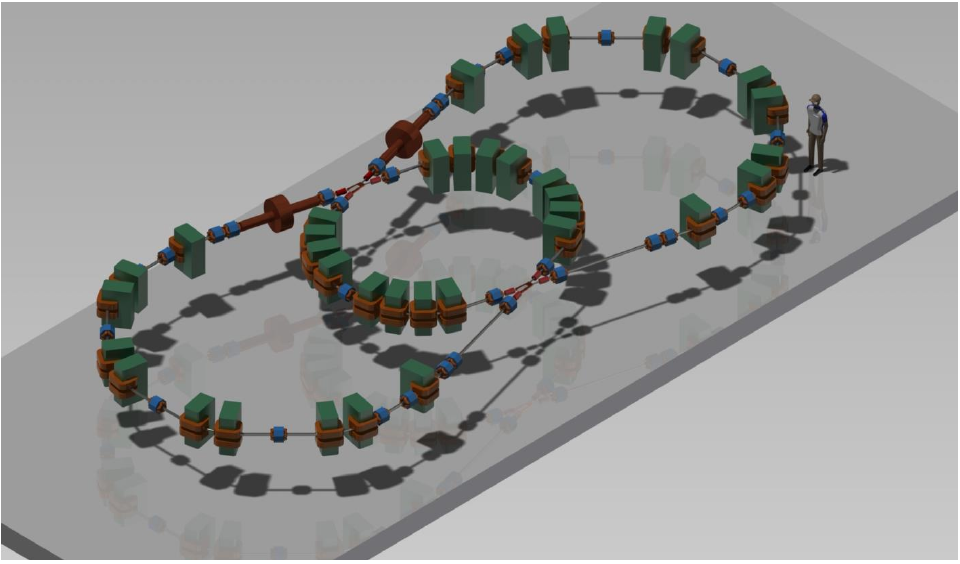
\includegraphics[width = 0.95\linewidth]{mumutron.png}
			\end{column}

			\begin{column}{0.5\linewidth}
				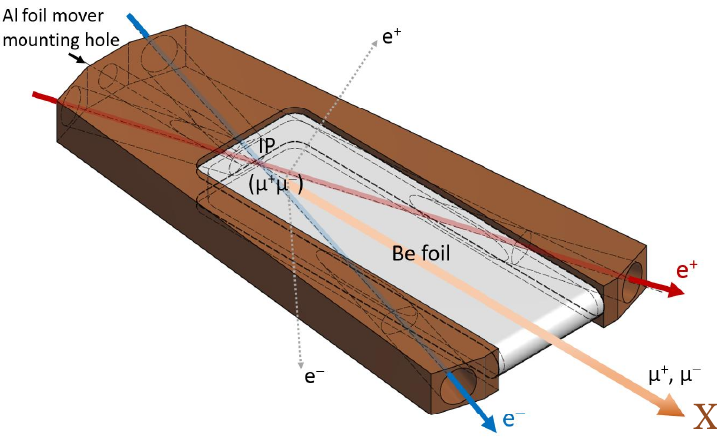
\includegraphics[width = 0.95\linewidth]{intreg.png}
			\end{column}
		\end{columns}
	\end{minipage}
\end{frame}

\begin{frame}
\begin{minipage}{\linewidth}
	\begin{columns}[T]
		\begin{column}{0.5\linewidth}
			\begin{flushleft}
				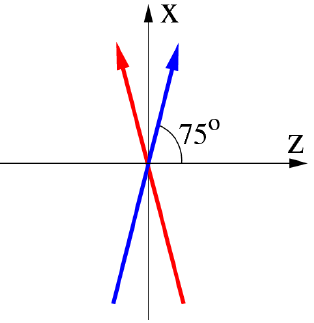
\includegraphics[width = 0.6\linewidth]{beams1.png}
			\end{flushleft}
		\end{column}

		\begin{column}{0.5\linewidth}
			Параметры коллайдера:\\
			$E_{\text{beam}} \approx 408\text{ MeV}$\\
			$E_{cm} \approx 211\text{ MeV}$\\
			Периметр $23\text{ м}$\\
			$\sigma_{E_{beam}}/E_{beam} \approx 7.8 \cdot 10^{-4}$\\
			$\sigma_{E_{cm}} \approx 0.4\text{ MeV}$\\
			$\alpha \approx 75^{\circ}$\\
			$\sigma_{\alpha} \approx 6.8 \cdot 10^{-4}$\\
			Светимость $8 \cdot 10^{31}\text{ $cm^{-2}c^{-1}$}$\\
			$\gamma = 3.86$\\
			$\beta = 0.966$\\
			Длина пролёта димюония $\ell = \gamma\beta c\tau = 2$ мм
		\end{column}
	\end{columns}
\end{minipage}
\end{frame}

\begin{frame}
	\centering
	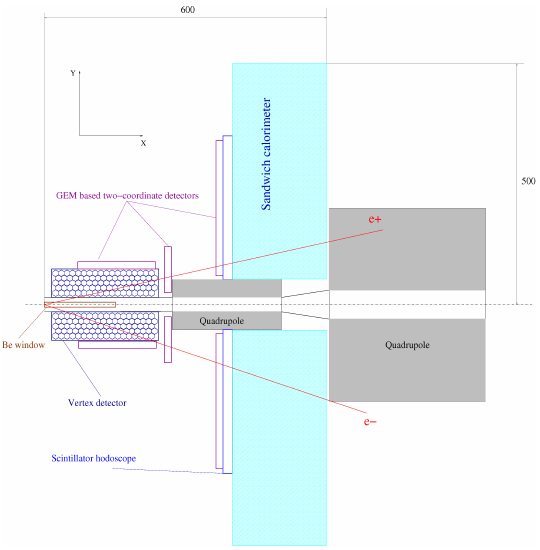
\includegraphics[height = \textheight]{eedet.png}
	\par
\end{frame}


\begin{frame}
	\begin{minipage}{\linewidth}
		\begin{columns}[T]
			\begin{column}{0.5\linewidth}
				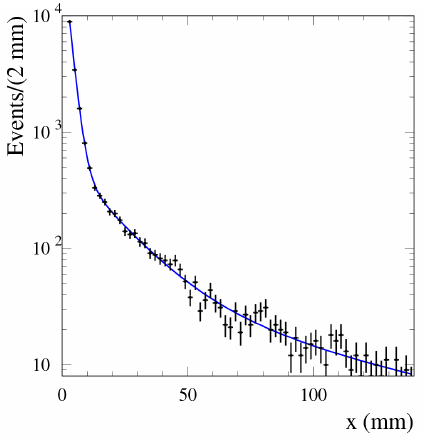
\includegraphics[scale = 0.5]{flight.png}
			\end{column}

			\begin{column}{0.5\linewidth}
				\fontsize{12pt}{20}\selectfont
				Измеряется $N_{1S}$ и $\ell_{1S}$.
				$\tau = \ell/(\gamma\beta c)$, $\sigma_{\ell} \sim 2\%$, $\sigma_{\gamma\beta} \sim 10^{-3}$
				$\rightarrow \sigma_{\tau} < 1\%$. $E$  необходимо выставлять с точностью лучше $\frac{1}{10}\sigma_E$.

				$N_{1S} \propto \Gamma_{ee}/\sigma_E$, поэтому для измерения $\Gamma_{ee}$
				с точностью порядка $1\%$ необходимо измерить $\sigma_E$ с точностью лучше $1\%$.
			\end{column}
		\end{columns}
	\end{minipage}
\end{frame}

\begin{frame}
	\centering
	$E$ и $\sigma_E$ измеряются по процессу $e^+e^- \rightarrow \mu^+\mu^-$.
	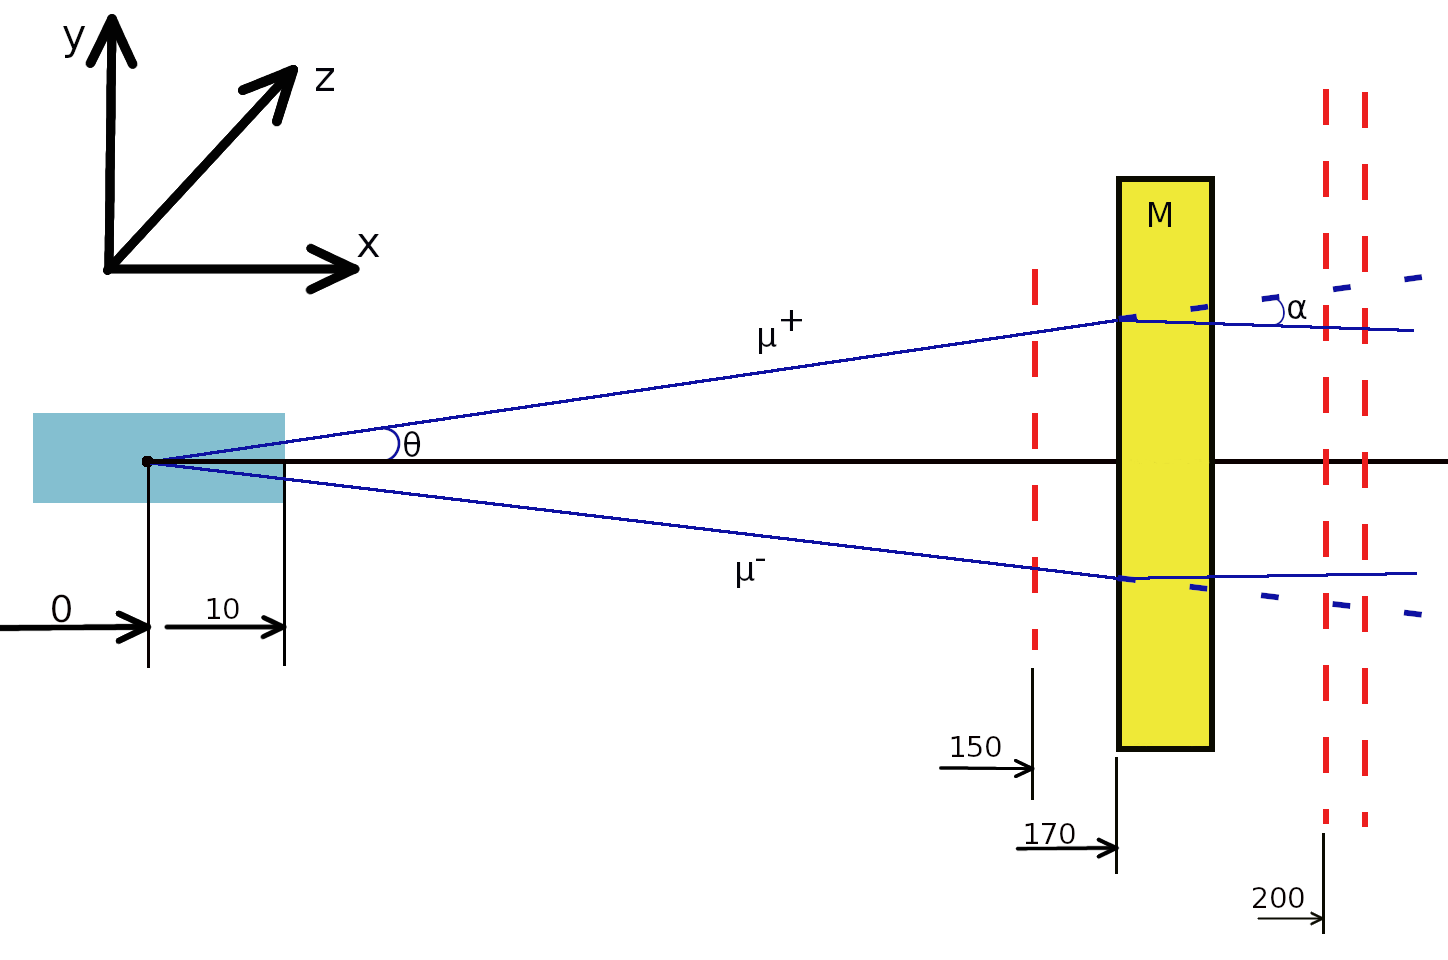
\includegraphics[width = 0.9\linewidth]{spectr.png}
	\par
\end{frame}

\begin{frame}
	\frametitle{Постановка эксперимента}
	1.) Сканирование порогового региона по энергии.\\
	2.) Установка пороговой энергии.\\
	3.) Набор статистики.\\
\end{frame}

\begin{frame}
	\frametitle{Расчёт сечения процесса $e^+e^- \rightarrow \mu^+\mu^-$ на пороге}
	\begin{minipage}{\linewidth}
		\begin{columns}[T]
			\begin{column}{0.3\linewidth}
				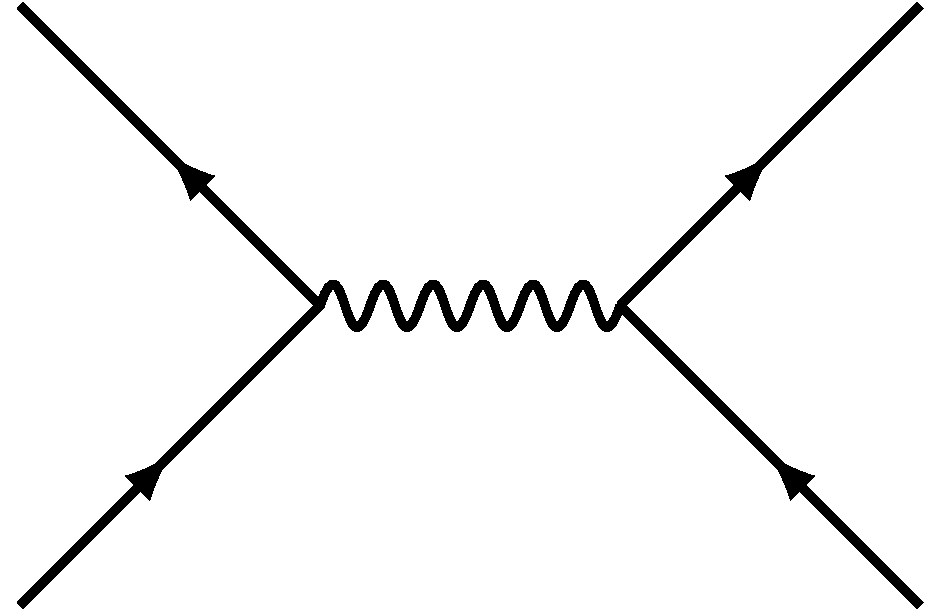
\includegraphics[width = 0.8\linewidth]{diagram1.pdf}
				\vspace{10pt}
				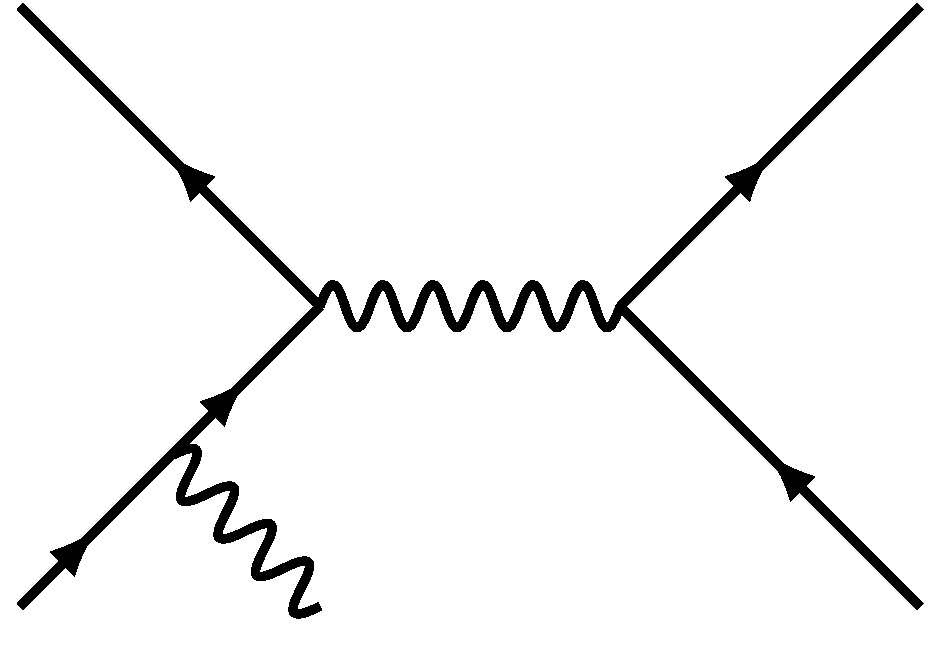
\includegraphics[width = 0.8\linewidth]{diagram2.pdf}
				\vspace{10pt}
				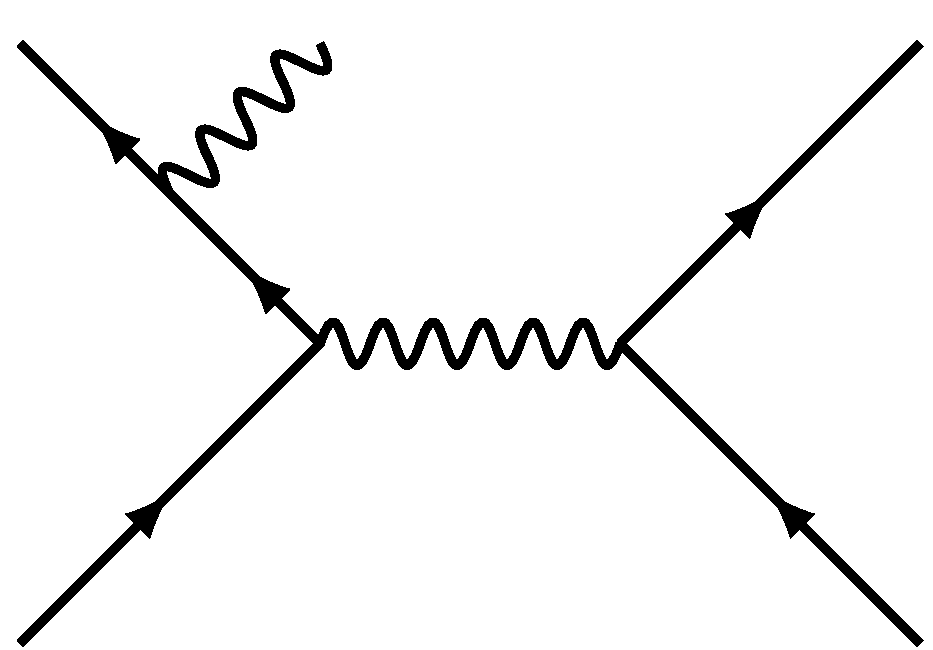
\includegraphics[width = 0.8\linewidth]{diagram4.pdf}
			\end{column}
			
			\begin{column}{0.3\linewidth}
				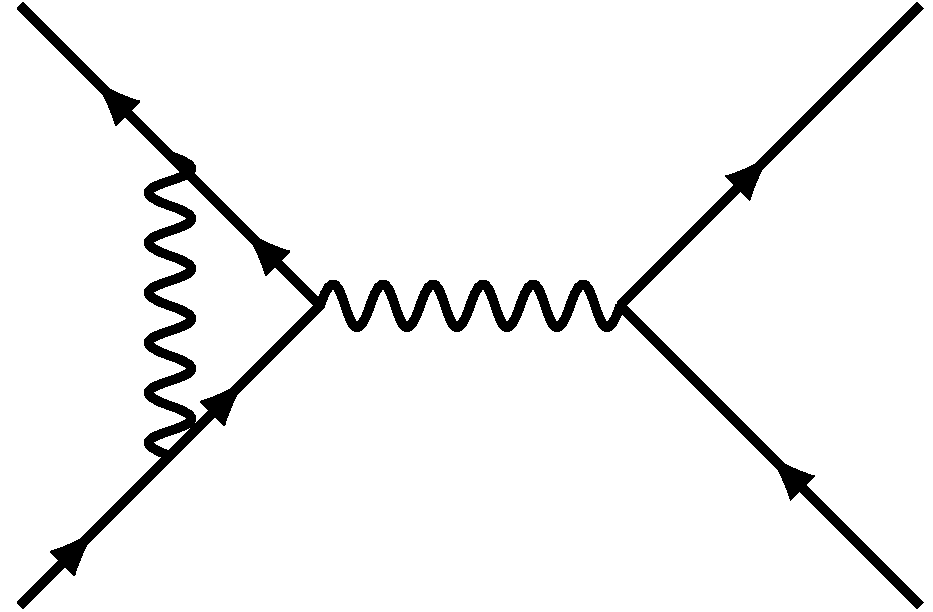
\includegraphics[width = 0.8\linewidth]{diagram5.pdf}
				\vspace{10pt}
				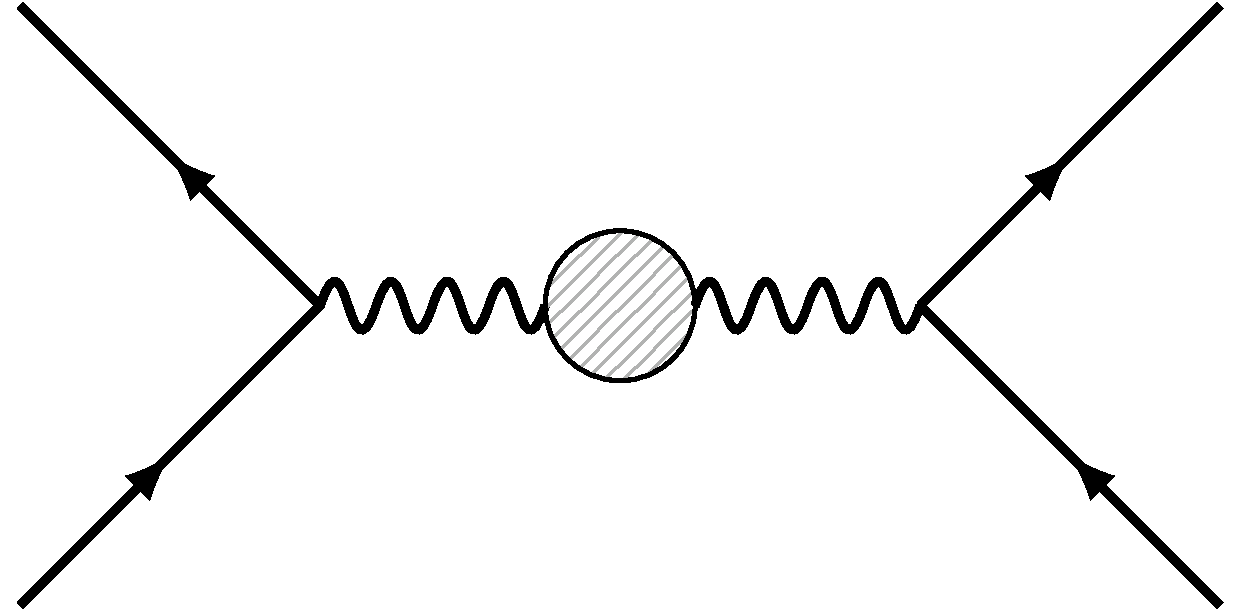
\includegraphics[width = 0.8\linewidth]{diagram3.pdf}
				\vspace{10pt}
				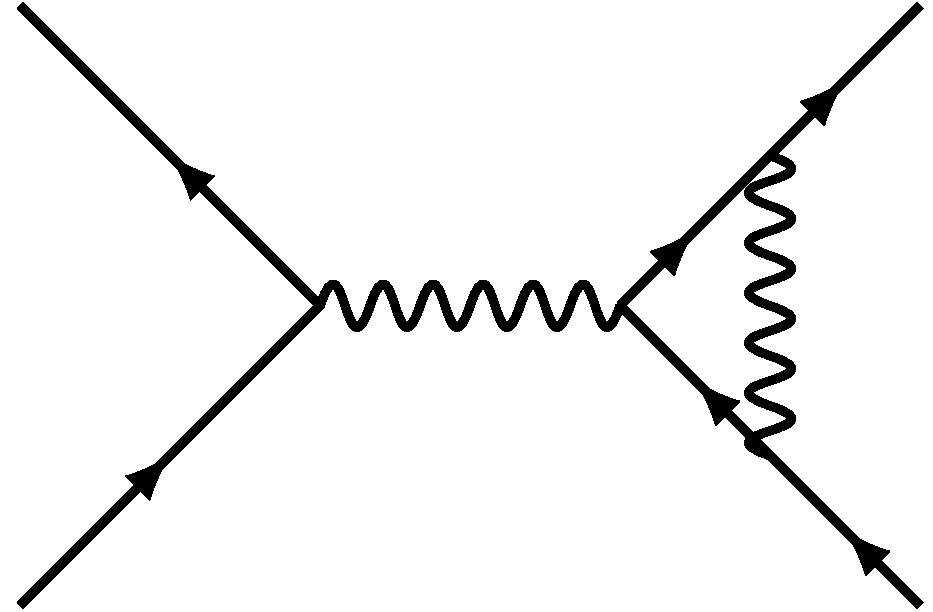
\includegraphics[width = 0.8\linewidth]{diagram6.pdf}
			\end{column}

			\begin{column}{0.3\linewidth}
				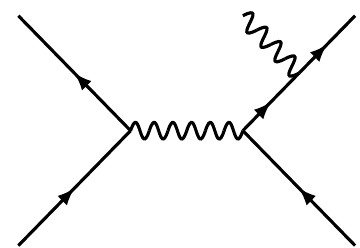
\includegraphics[width = 0.8\linewidth]{diagram7.png}
				\vspace{10pt}
				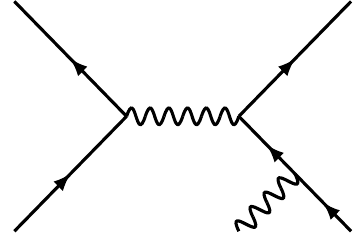
\includegraphics[width = 0.8\linewidth]{diagram8.png}
			\end{column}
		\end{columns}
	\end{minipage}
\end{frame}

\begin{frame}
	\fontsize{12pt}{30}\selectfont
$\sigma_B(E) = \frac{2\pi\alpha\beta}{E^2}(1 - \frac{\beta^2}{3})C(E).$\\
				
$C(E)$ - фактор Зоммерфельда-Гамова-Сахарова.\\
		
$C(E) = \frac{\eta}{1 - e^{-\eta}}, \quad \eta = \frac{\pi\alpha}{\beta}.$\\
	
$\sigma_{\text{vis}} = \displaystyle \int_0^{x_{max}} dx \sigma_B(E\sqrt{1 - x})W(E, x).$\\ 
				
$x = 2E_{\gamma}/E, \quad x_{max} = 1 - 4m_e^2/E^2.$\\
				
$\sigma_{exp} = 
\frac{1}{\sqrt{2\pi}\sigma_E}\displaystyle \int_{-\infty}^{\infty} dE \sigma_{\text{vis}}(E)\text{exp}\left[-\frac{(E - E_0)^2}{2\sigma_E^2}\right]$
\end{frame}

\begin{frame}
\begin{minipage}{\linewidth}
\begin{columns}
\begin{column}{0.6\linewidth}
\centering
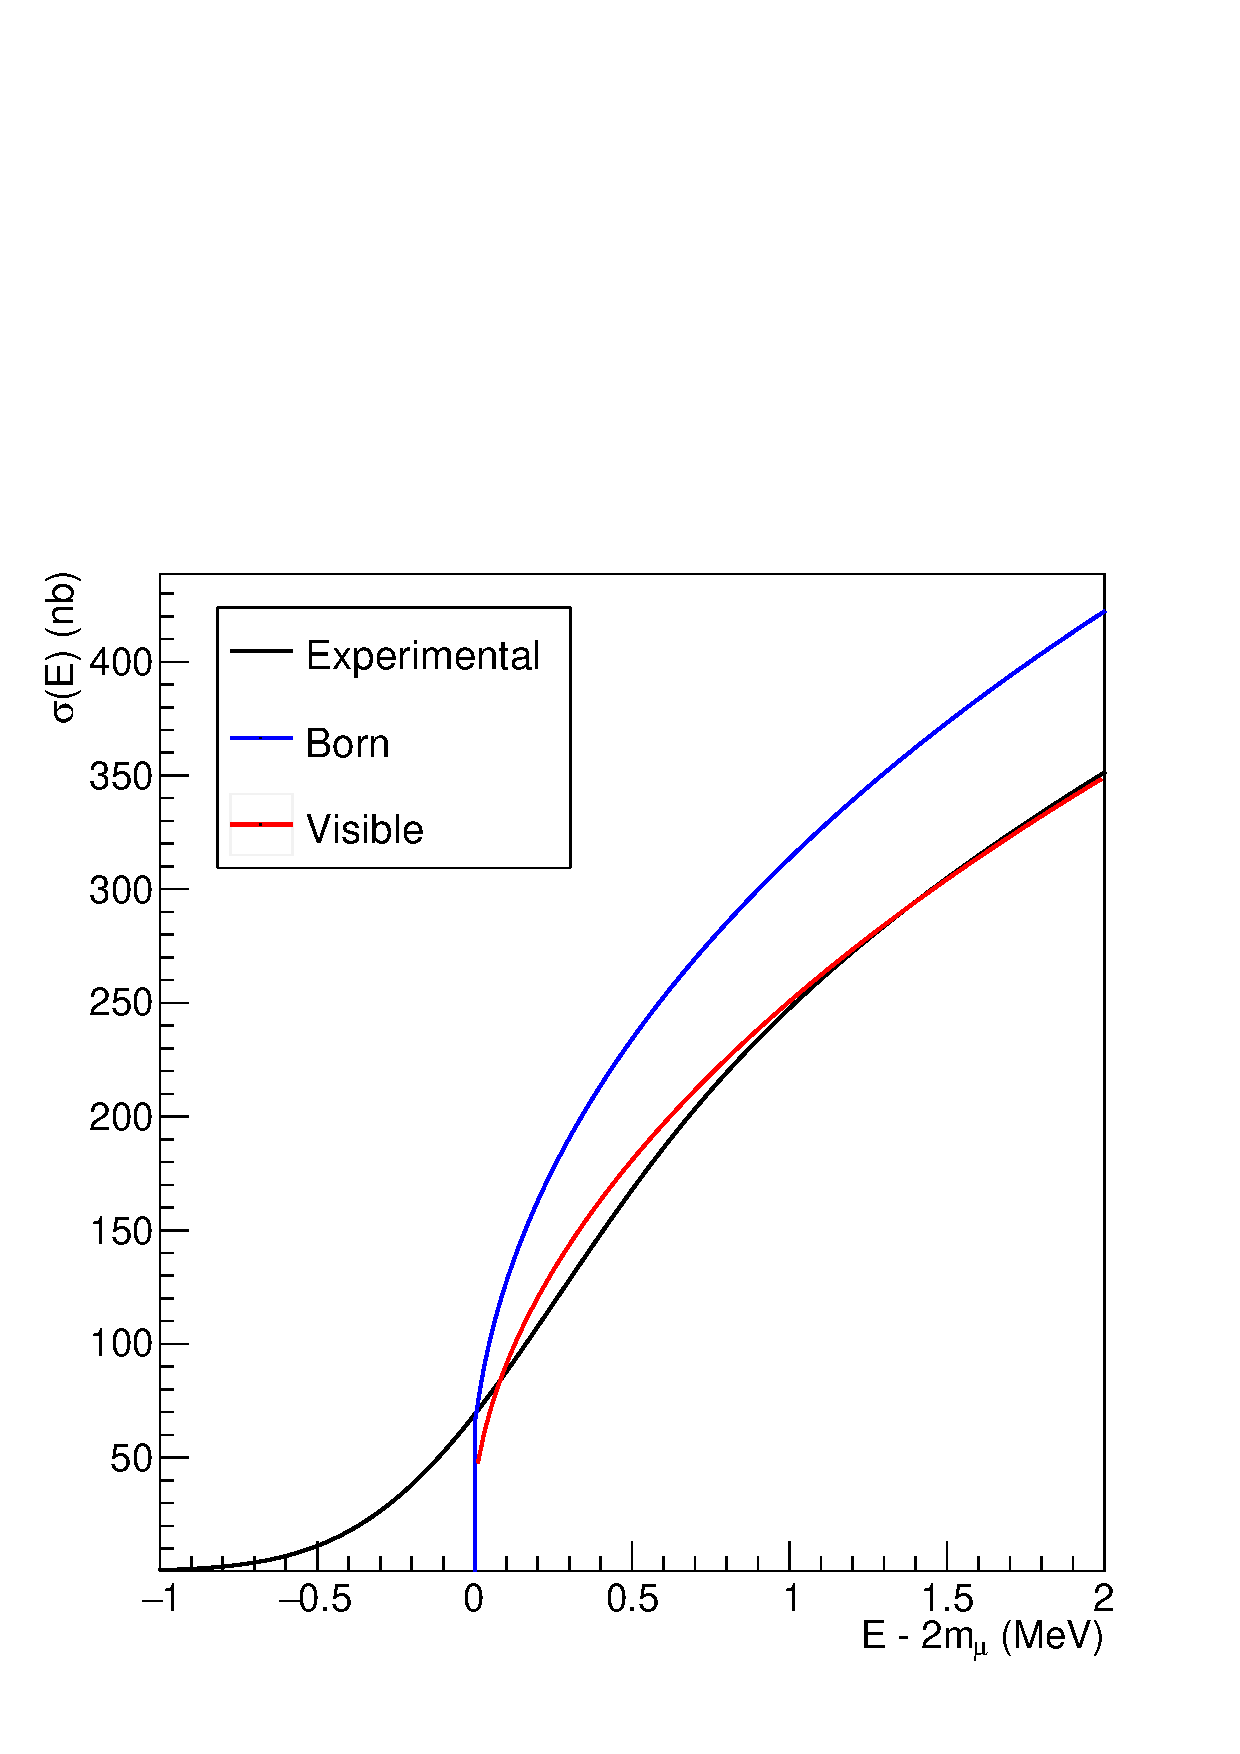
\includegraphics[scale = 0.38]{secs.pdf}
\par
\end{column}

\begin{column}{0.4\linewidth}
$\sigma_B(2m_{\mu}) = 65$ нб.
$\sigma_{vis}(2m_{\mu}) = 44$ нб.
$\sigma_{exp}(2m_{\mu}) = 66$ нб.
\end{column}
\end{columns}
\end{minipage}
\end{frame}

\begin{frame}
	\frametitle{Сканирование по энергии}

	Сканирование проводится по трём точкам. Теоретическое сечение параметризуется сдвигом энергии от порога $\Delta E$,
	энергетическим разбросом $\sigma_E$ и эффективностью регистрации $\epsilon$.
	\begin{equation}
		\sigma = \sigma_{exp}(E + \Delta E, \sigma_E)\epsilon.
	\end{equation}

	После этого генерируется три значения $N$ для проектных значений параметров:
	\begin{equation}
		N_i = L\sigma_{exp}(E_i; \sigma_E=400\mbox{ кэВ})t,\;i=1,3. 
	\end{equation}
	$t = 3600$ с. После этого проводится подгонка полученных значений теоретическим сечением. Точки по энергии затем варьируются
	так, чтобы ошибка подгонки была минимальной.
\begin{table}
\begin{tabular*}{\textwidth}{ @{\extracolsep{\fill}}c c  c  c }
\hline
$E$ & $2m_{\mu} - 1.5\sigma_E$ & $2m_{\mu} + \sigma_E$ & $2m_{\mu} + 2$ МэВ\\
\hline
$\sigma$(нб) & 6.97 & 147.6 & 351.4\\
\hline
$N$ & 2007 & 42496 & 101195\\
\hline
\end{tabular*}
\par
\end{table}
\end{frame}

\begin{frame}
\begin{minipage}{\linewidth}
\begin{columns}
\begin{column}{0.6\linewidth}
\centering
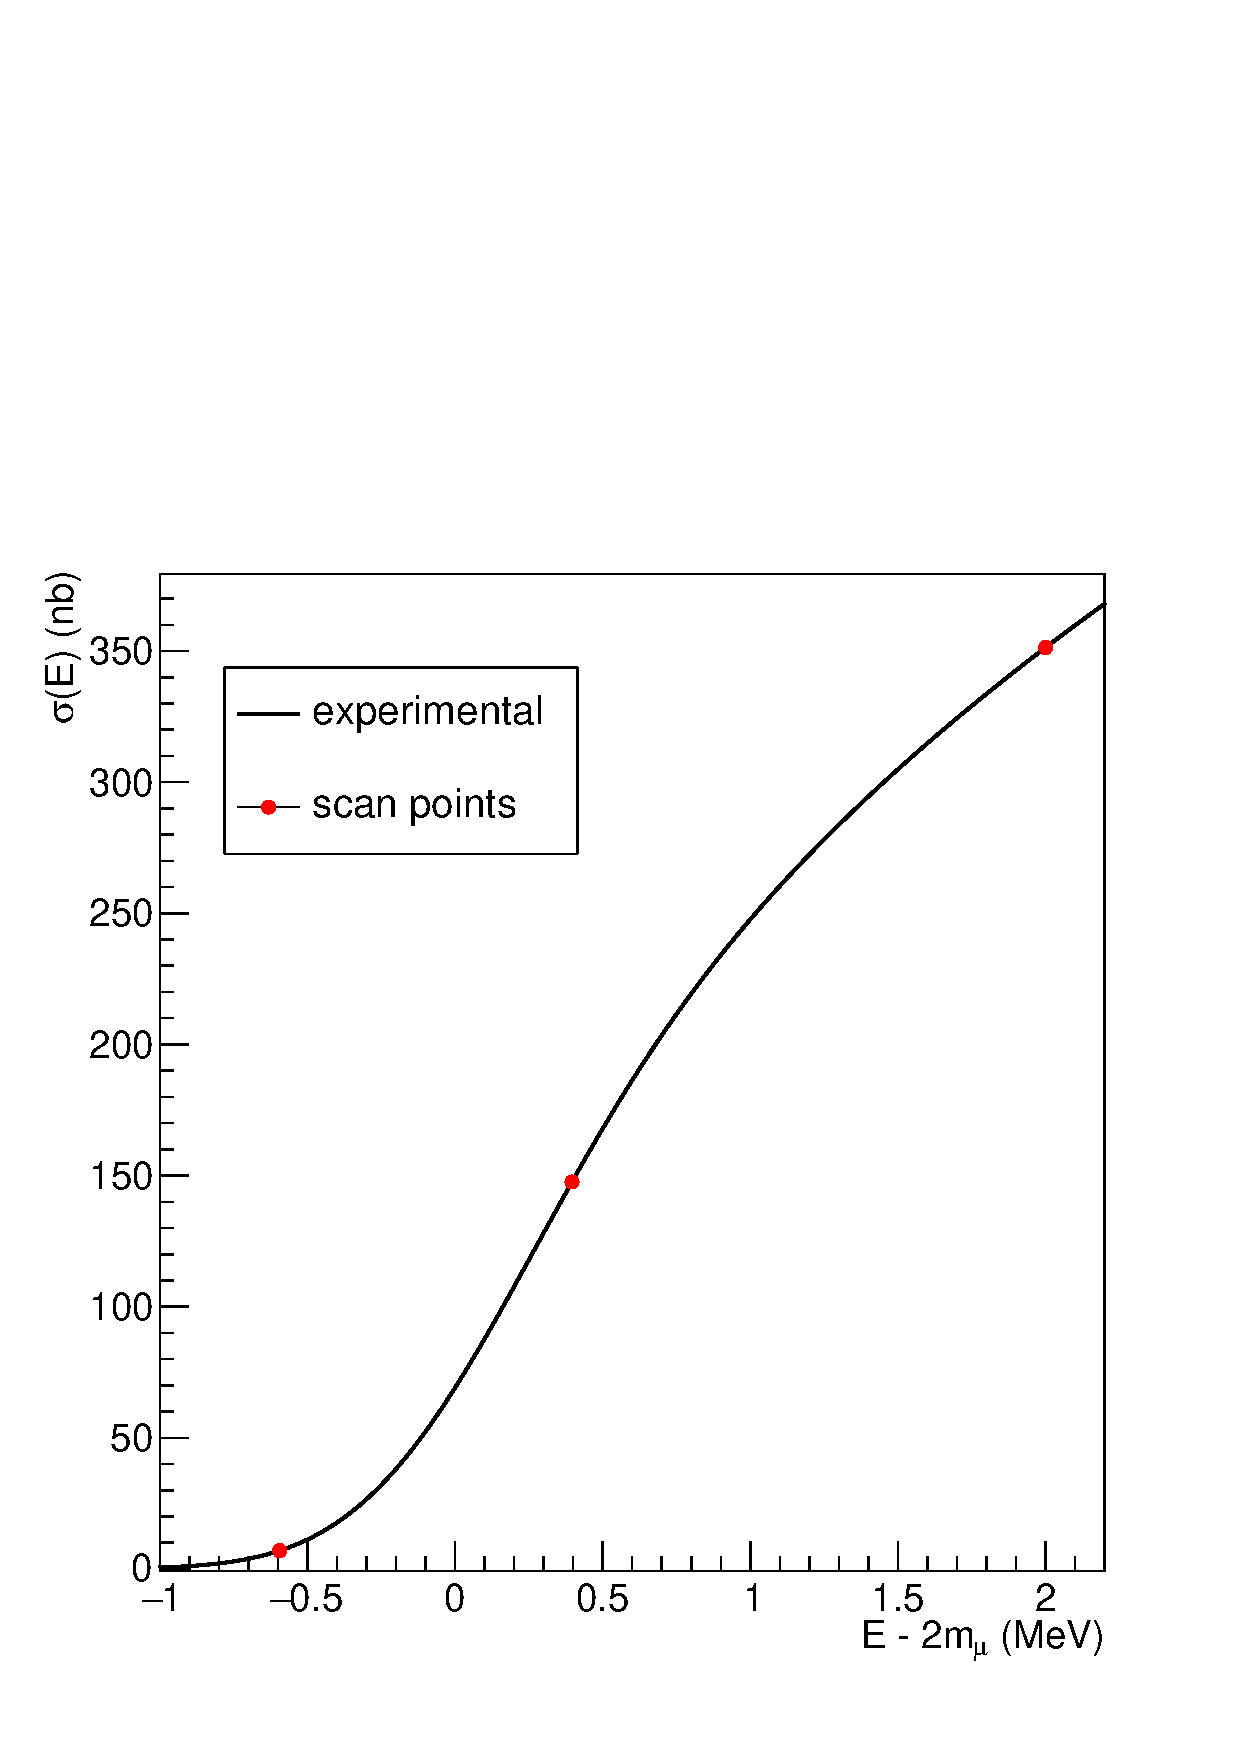
\includegraphics[scale = 0.38]{scan.pdf}
\par
\end{column}

\begin{column}{0.4\linewidth}
\fontsize{7pt}{10}\selectfont
Точность измерения $E = 5$ кэВ.\\
Точность измерения $\sigma_E = 4$ кэВ.
\end{column}
\end{columns}
\end{minipage}
\end{frame}

\begin{frame}
	\frametitle{Контроль энергии в системе центра масс}
	\begin{minipage}{\linewidth}
		\begin{columns}[T]
			\begin{column}{0.63\linewidth}
				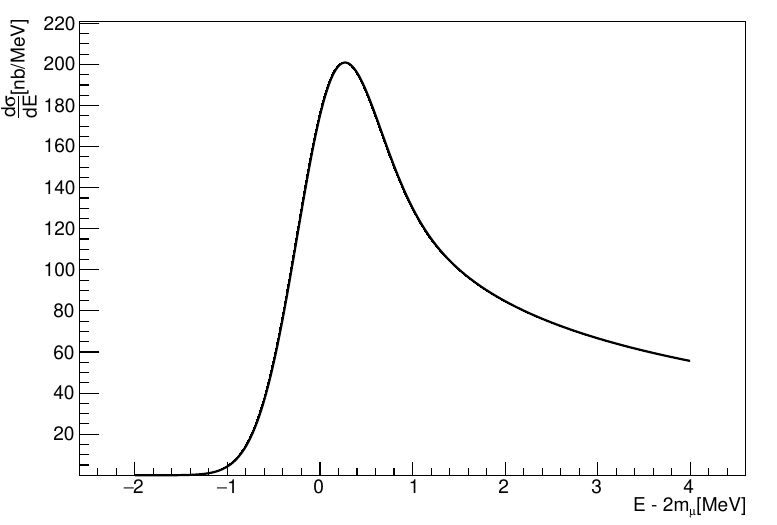
\includegraphics[scale = 0.37]{deriv.png}
			\end{column}

			\begin{column}{0.37\linewidth}
				\fontsize{10pt}{20}\selectfont
				$\Delta E=\Delta \sigma_{exp}(E)\left( \frac{d\sigma}{dE} \right ) ^{-1}$\\
				$\Delta\sigma = \frac{\sqrt{N}}{Lt} = \sqrt{\frac{\sigma}{Lt}}$\\
				$\Delta E = \sqrt{\frac{\sigma}{Lt}}\left( \frac{d\sigma}{dE} \right)^{-1}$
				Контроль $E$ с точностью $60$ кэВ/сутки.
			\end{column}
		\end{columns}
	\end{minipage}

\end{frame}

\begin{frame}
	\frametitle{Измерение разброса по энергии}

	\centering
	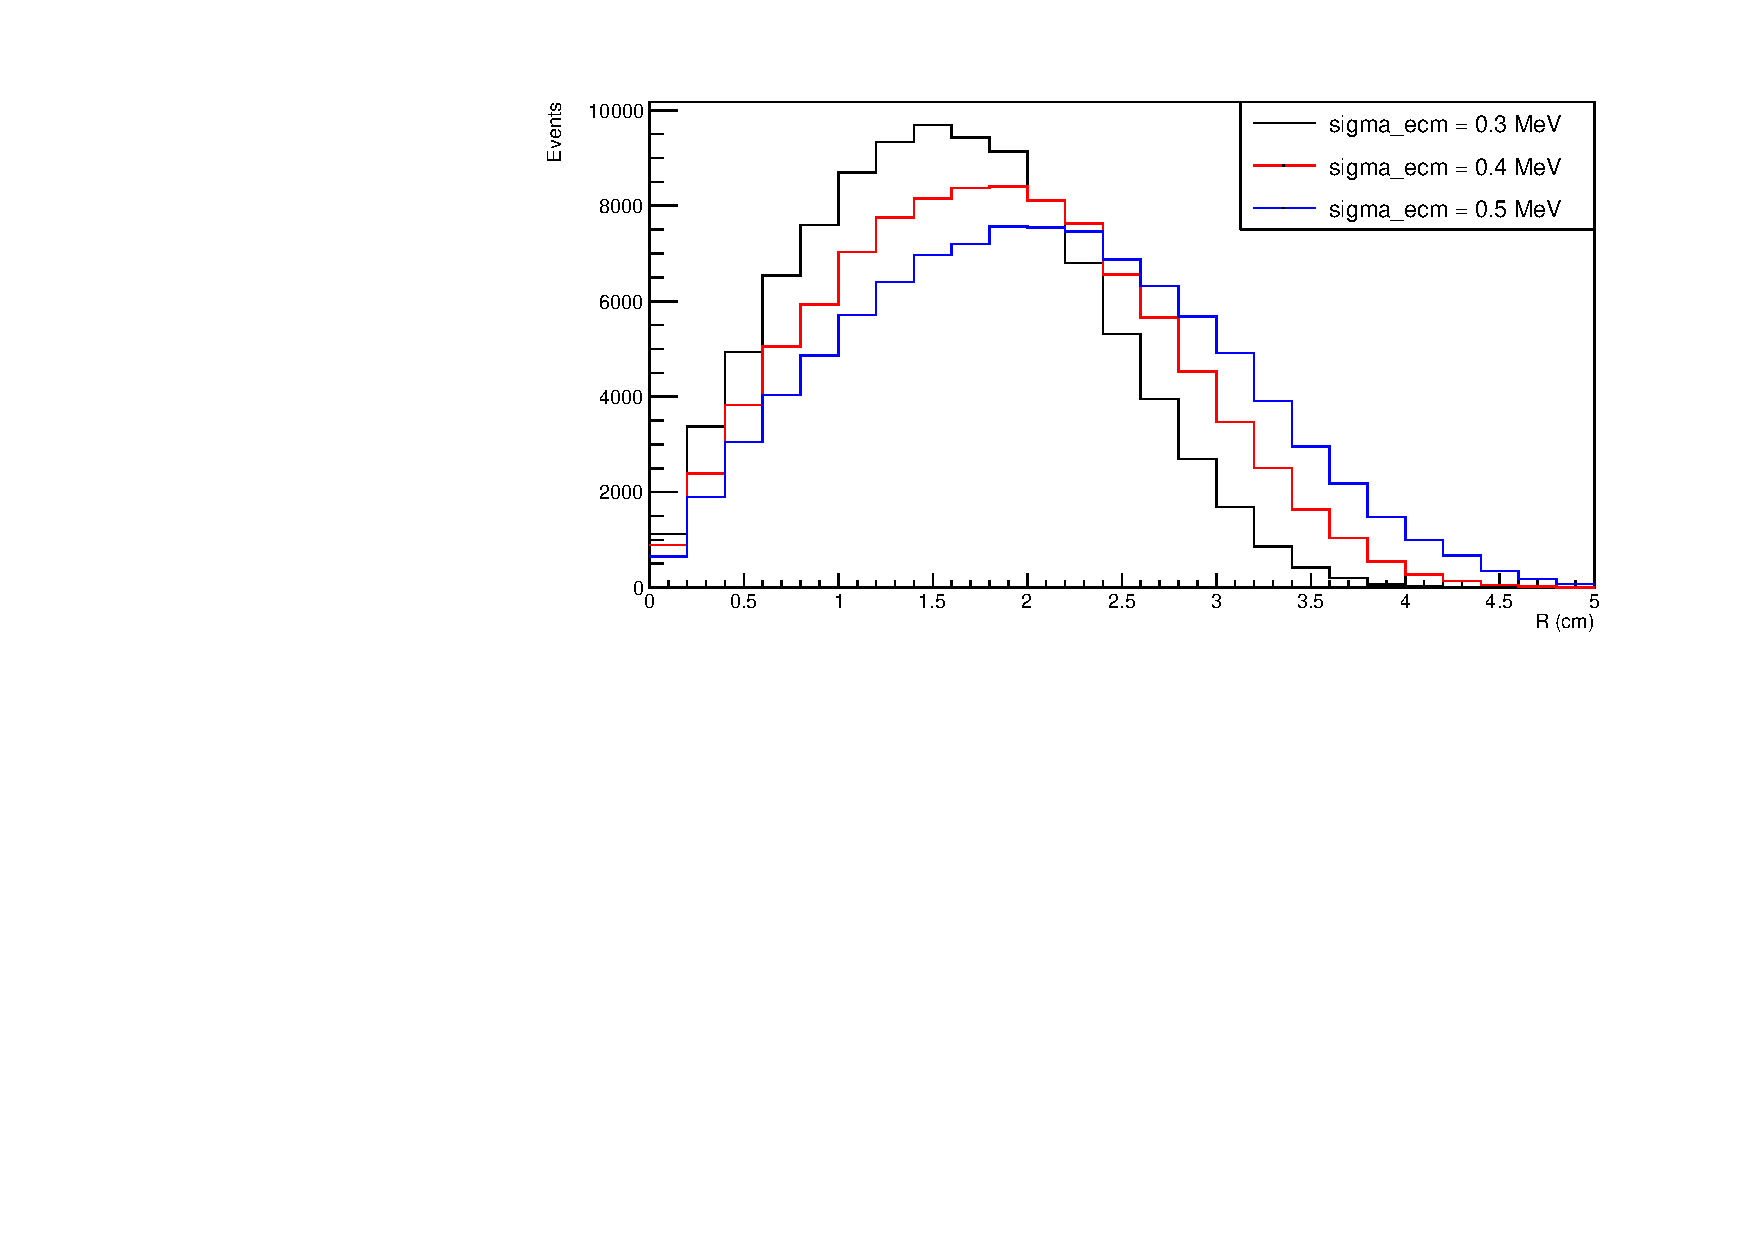
\includegraphics[scale = 0.6]{hists.pdf}
	\par
	\end{frame}

\begin{frame}

	\centering
	$\sigma_E$ контролируется с точностью $\sim 3$ кэВ/час.
	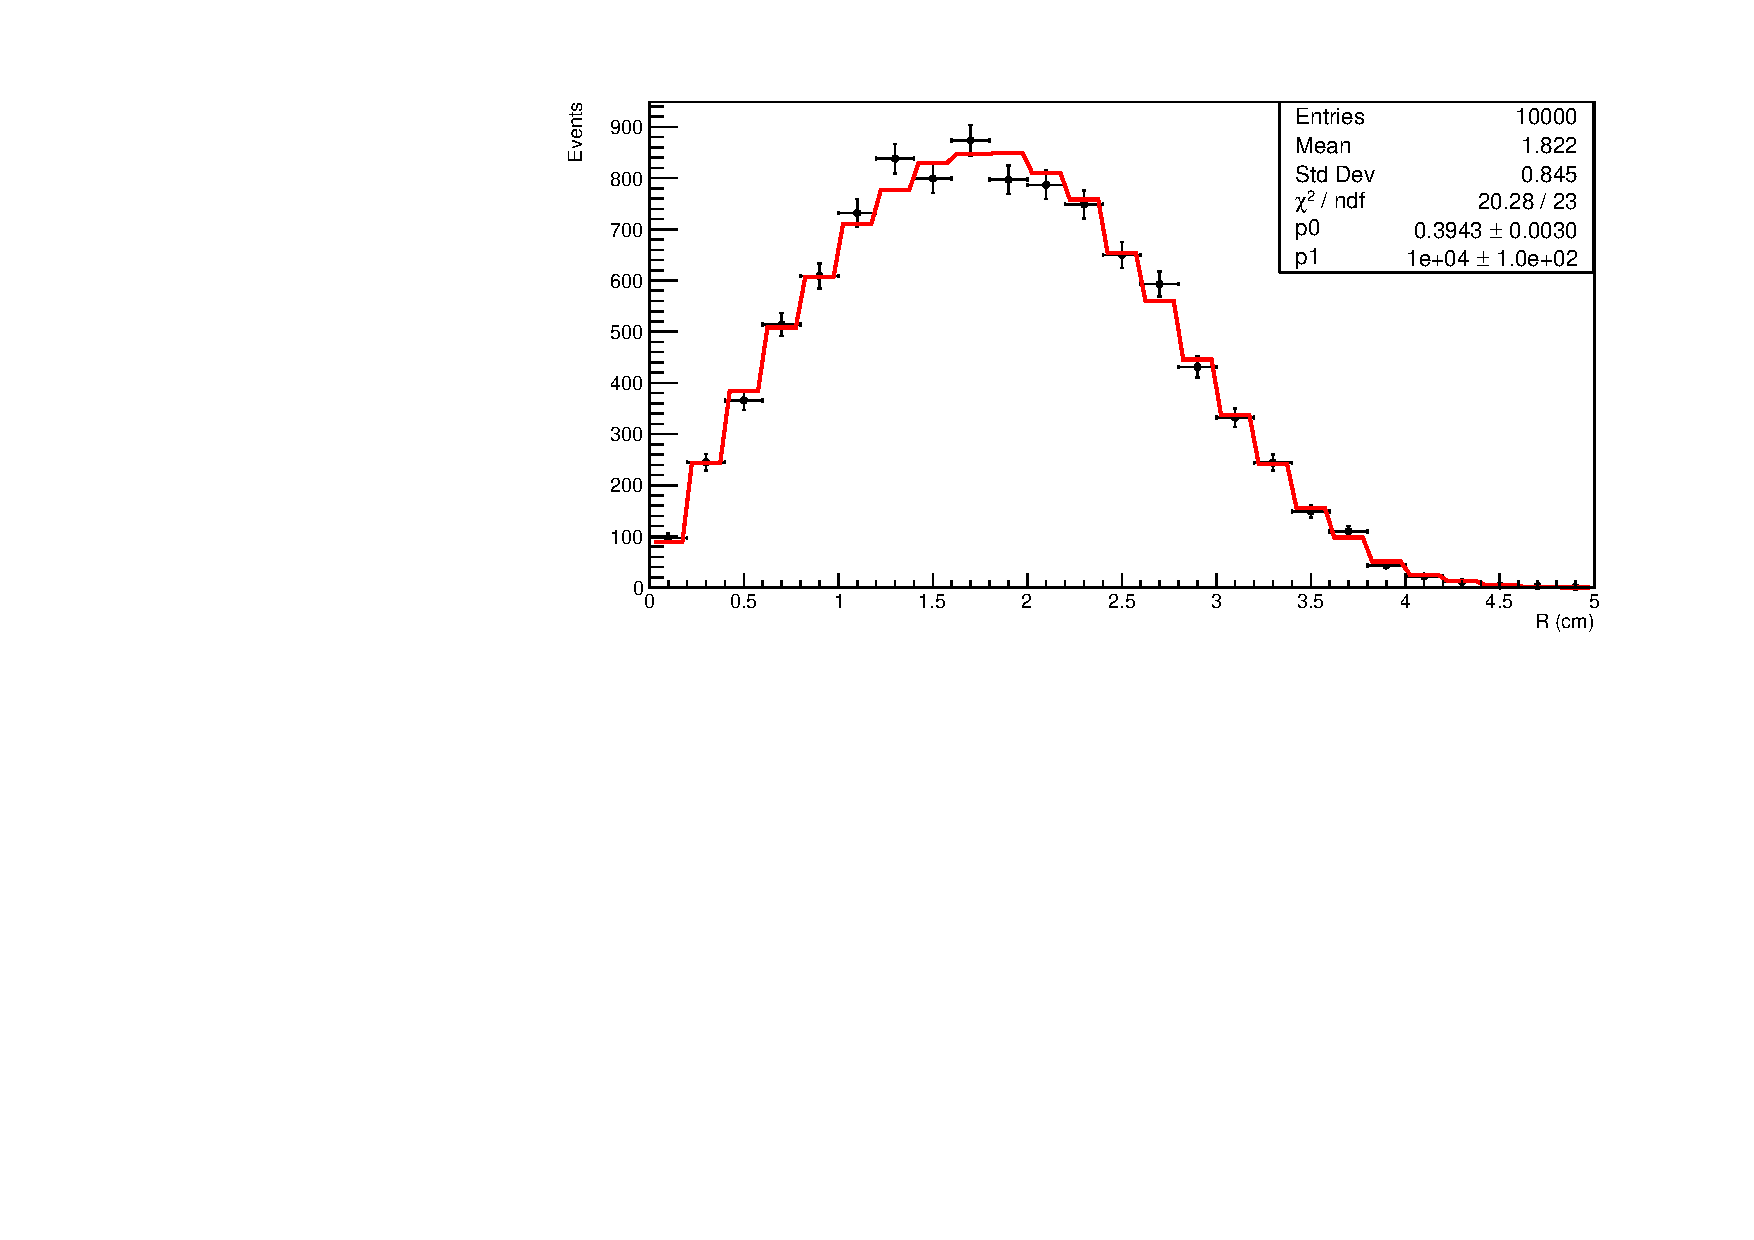
\includegraphics[height = 0.8\textheight]{res.pdf}
	\par
\end{frame}

\begin{frame}
	\frametitle{Заключение}
	\fontsize{8pt}{7.2}\selectfont
	Цель работы: разработать методику измерения энергии в системе центра масс и её разброса на коллайдере мюмютрон.
	Для этого необходимо сделать:
	\begin{itemize}
		\item Расчёт сечения процесса $e^+e^- \rightarrow \mu^+\mu^-$ на пороге
		\item Расчёт зависимости производной сечения процесса по энергии от энергии
		\item Написание программы моделирования процесса с учётом многократного рассеяния и точности детектора 
	\end{itemize}
	Результаты:
	\begin{itemize}
		\item Проведён расчёт сечения процесса $e^+e^- \rightarrow \mu^+\mu^-$ и его производной в припороговой области энергии
		\item Определены точки для сканирования: $2m_{\mu} - 1.5\sigma_E$, $2m_{\mu} + \sigma_E$, $2m_{\mu} + 2\text{ МэВ}$.
		\item Определена точность измерения энергии и энергетического разброса при сканировании, 
			которая составила $5$ кэВ и $4$ кэВ соответственно.
		\item Оценена точность контроля энергии при часовом наборе данных, составляющая $\approx 3$ кэВ 
		\item Проведено Монте-Карло моделирование процесса $e^+e^- \rightarrow \mu^+\mu^-$ вблизи порога
		\item Определена точность контроля энергетического разброса, которая составляет $\backsim 3$ кэВ/час
	\end{itemize}

\end{frame}

\end{document}
